\documentclass[aspectratio=1610]{beamer}
\usepackage[utf8]{inputenc}
\usepackage[T1]{fontenc}
\usepackage[german]{babel}
\usepackage[useregional]{datetime2}
\usepackage[nameinlink]{cleveref}
\usepackage[section]{placeins}
\usepackage{xcolor}
\usepackage{graphicx}
\usepackage{csquotes}
\usepackage{amsmath} % for $\text{}$
\usepackage{pflichtenheft}
\usepackage{enumitem}
\setlist{nosep}

\newcommand\urlpart[2]{$\underbrace{\text{\texttt{#1}}}{\text{#2}}$}
\raggedbottom
\crefname{figure}{Abb}{Abb}

\newcommand\producttitle{treff.}
\hypersetup{
	pdftitle={Pflichtenheft: \producttitle},
	bookmarks=true,
}


% header & footer
\usepackage{scrlayer-scrpage}
%\lofoot{\today}
%\refoot{\today}
\pagestyle{scrheadings}

\title{
\includegraphics[width = 50mm]{images/logo_crop.png}}
\subtitle{\huge Pflichtenheft}
\author{Lukas Dippon
	\and Jens Kienle
	\and Matthias Noll
	\and Fabian Röpke
	\and Tim Schmidt
	\and Simon Vögele}

\begin{document}

	\begin{frame}[plain]
	\maketitle
	\end{frame}

	\begin{frame}[plain]
		\frametitle{Aufgabenstellung}
		\begin{itemize}
			\item[--] write your favourite android app
			\item
			\item [--]Client-/Server Applikation
			\item
			\item[--] Go-App zur Organisation in Gruppen
		\end{itemize}
	\end{frame}

	\begin{frame}[plain]
		\frametitle{Selbstgesetzte Rahmenbedingungen}
		\begin{itemize}
			\item[--] Anwendung, die wir auch  selbst benutzen würden
			\item
			\item[--] keine closed source dependencies
			\item
			\item [--]kein KIT Fokus
			\item
			\item [--]viele Datenschutz- und Shareoptionen
		\end{itemize}
	\end{frame}

	\begin{frame}[plain]
	\frametitle{1. Konten}
	\begin{minipage}{0.5\textwidth}
	\setlength{\fboxsep}{0pt}% space between border and image
	\setlength{\fboxrule}{1pt}% width of border
	\fbox{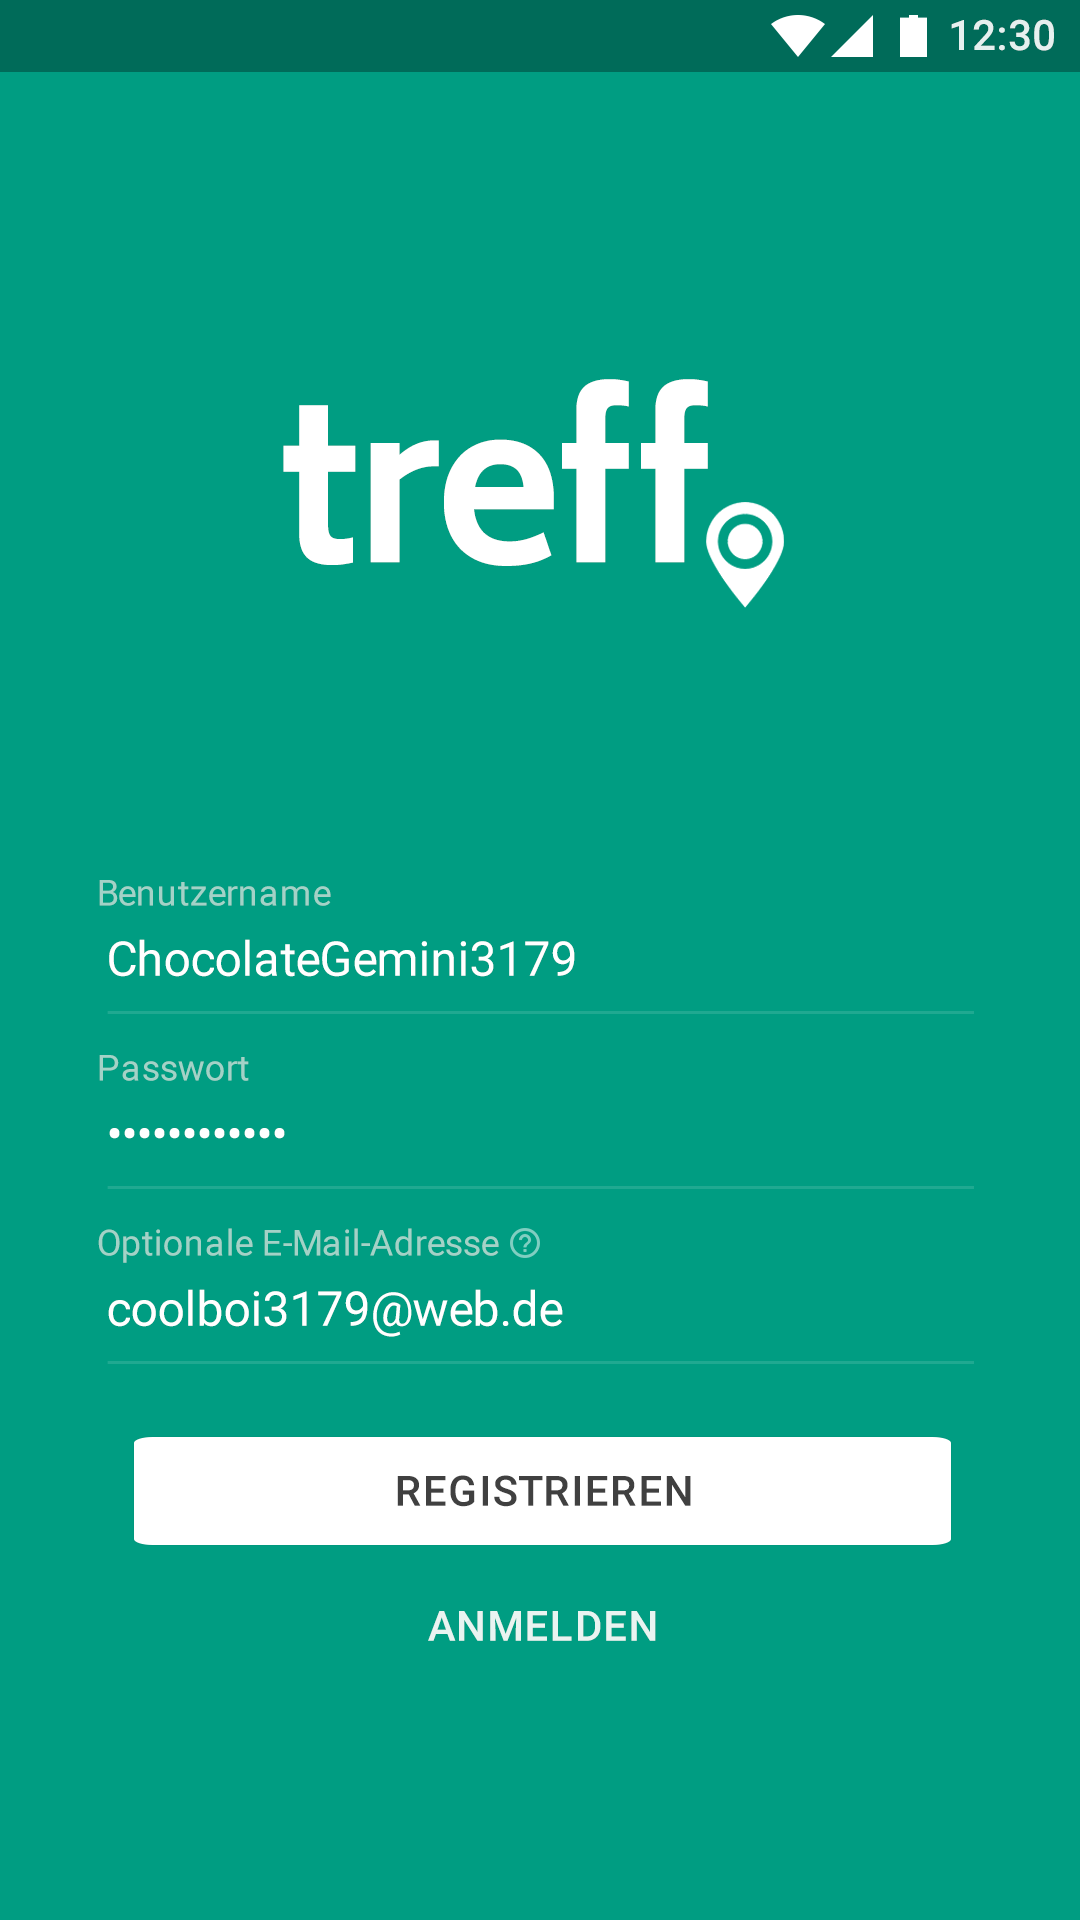
\includegraphics[width = 45mm]{images/gui-mockups/register.png}}
	\captionsetup{labelformat=empty}
	\centering
	\captionof{figure}{Registrieren}
	\end{minipage}%
	\begin{minipage}{0.5\textwidth}
		\textbf{Überlegungen}
		\begin{itemize}
			\item<2->[--] Google-Login?
			\item<2->[--] Nutzernamen ändern?
		\end{itemize}
	\end{minipage}
	\end{frame}

	%%%%%%%%%%%%%%%%%%%%%%%%%%%%%%%%%%%%%%%%%%%%%%%%%%%

	\begin{frame}[plain]
	\frametitle{2. Freunde und Gruppen}
	\begin{minipage}{0.5\textwidth}
		\setlength{\fboxsep}{0pt}% space between border and image
		\setlength{\fboxrule}{1pt}% width of border
		\fbox{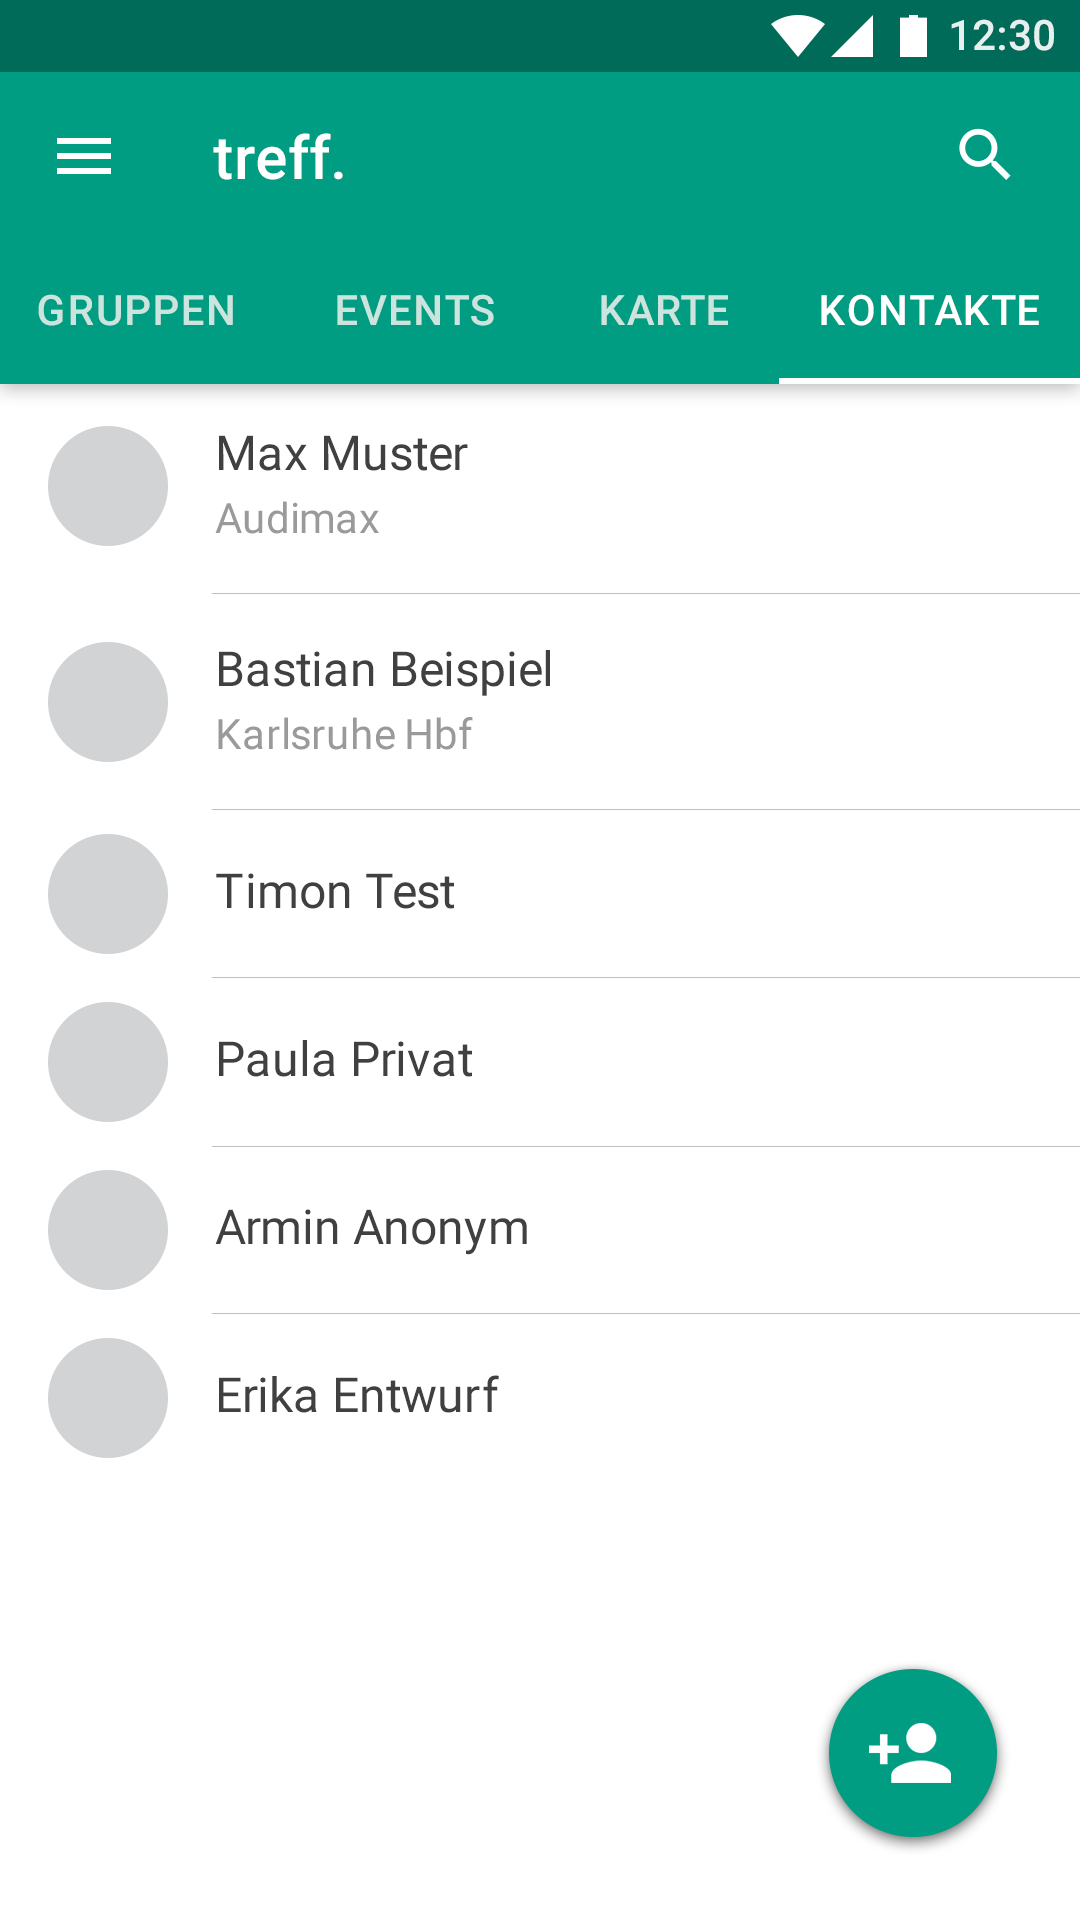
\includegraphics[width = 45mm]{images/gui-mockups/home_friends.png}}
		\captionsetup{labelformat=empty}
		\centering
		\captionof{figure}{Freunde}
	\end{minipage}%
	\begin{minipage}{0.5\textwidth}
		\begin{itemize}
			\setlength\itemsep{0.3em}
			\item[--] Freunde als Liste
			\item[--]	Gegenseitiges Hinzufügen über Suchfunktion
		\end{itemize}
	\end{minipage}%
	\end{frame}

	\begin{frame}[plain]
	\frametitle{2. Freunde und Gruppen}
		\begin{minipage}{0.5\textwidth}
			\setlength{\fboxsep}{0pt}% space between border and image
			\setlength{\fboxrule}{1pt}% width of border
			\fbox{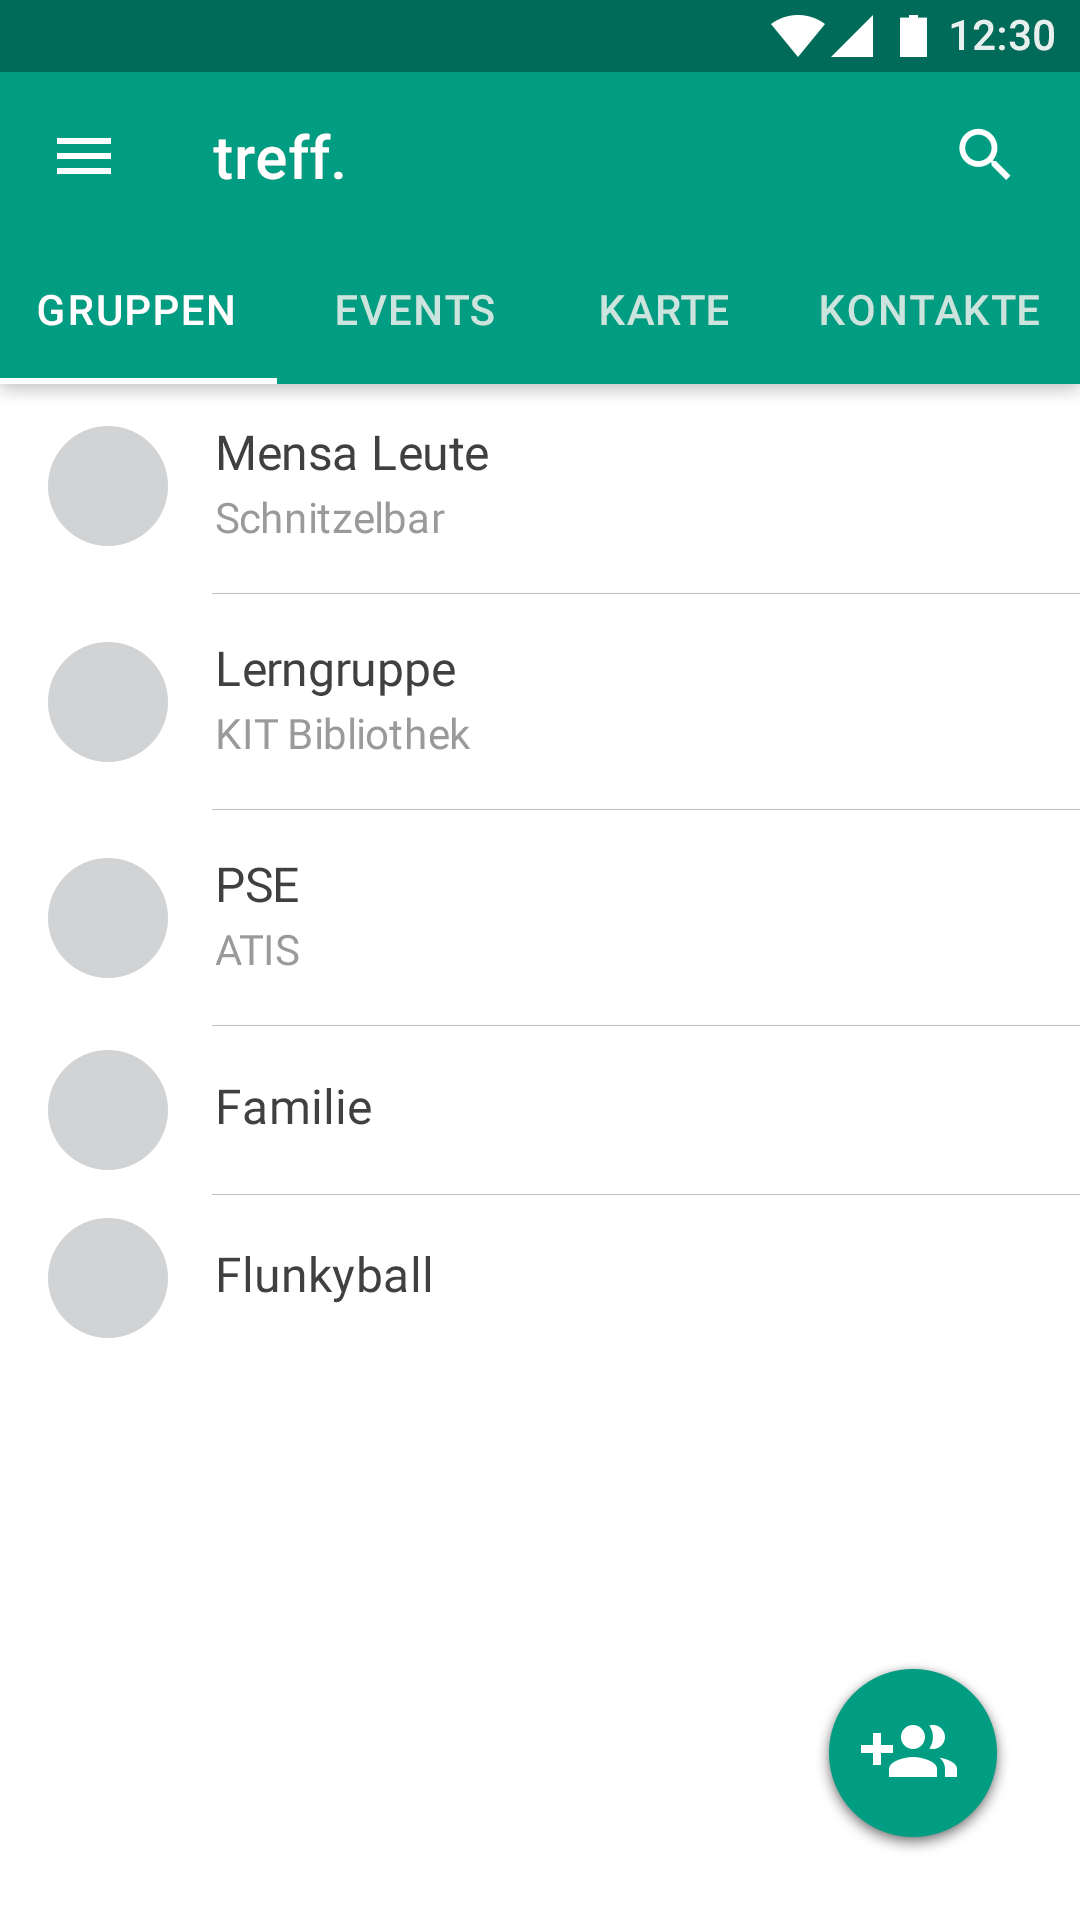
\includegraphics[width = 45mm]{images/gui-mockups/home_groups.png}}
			\captionsetup{labelformat=empty}
			\centering
			\captionof{figure}{Gruppen}
		\end{minipage}%
		\begin{minipage}{0.5\textwidth}
			\begin{itemize}
				\setlength\itemsep{0.3em}
				\item[--] Erstellen von Gruppen
				\item[--] Hinzufügen und Entfernen von Mitgliedern
			\end{itemize}
		\end{minipage}%
	\end{frame}

	\begin{frame}[plain]
	\frametitle{3. Darstellung von Standorten}
		\begin{minipage}{0.5\textwidth}
			\setlength{\fboxsep}{0pt}% space between border and image
			\setlength{\fboxrule}{1pt}% width of border
			\fbox{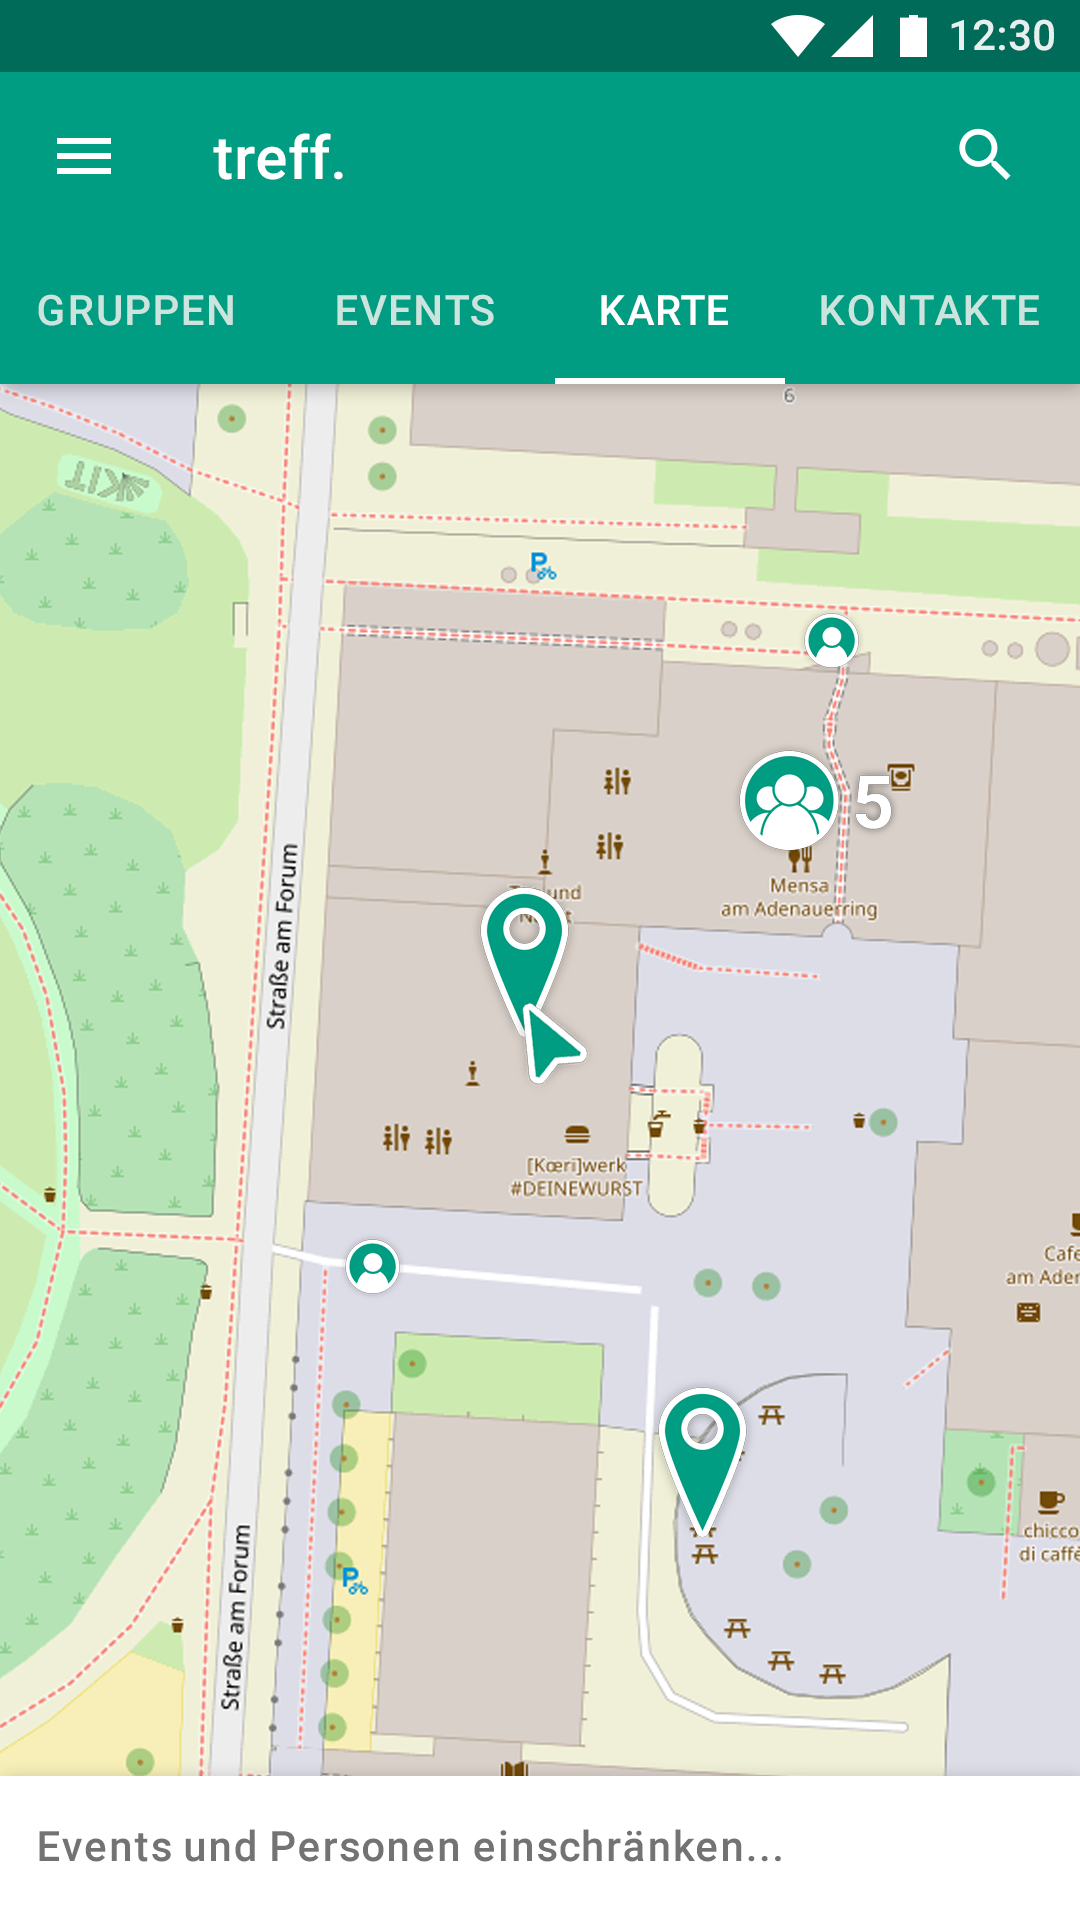
\includegraphics[width = 45mm]{images/gui-mockups/home_map.png}}
			\captionsetup{labelformat=empty}
			\centering
			\captionof{figure}{Umgebungskarte}
		\end{minipage}%
		\begin{minipage}{0.5\textwidth}
			\begin{itemize}
				\setlength\itemsep{0.3em}
				\item[--] Karte der eigenen Umgebung
				\item[--] Eigener Standort im Zentrum
				\item[--] Standorte von Freunden werden angezeigt
				\item[--] Zusammenfassung von Standorten zu Gruppierungen
			\end{itemize}
		\end{minipage}%
	\end{frame}

	\begin{frame}[plain]
	\frametitle{3. Darstellung von Standorten}
		\begin{minipage}{0.5\textwidth}
			\setlength{\fboxsep}{0pt}% space between border and image
			\setlength{\fboxrule}{1pt}% width of border
			\fbox{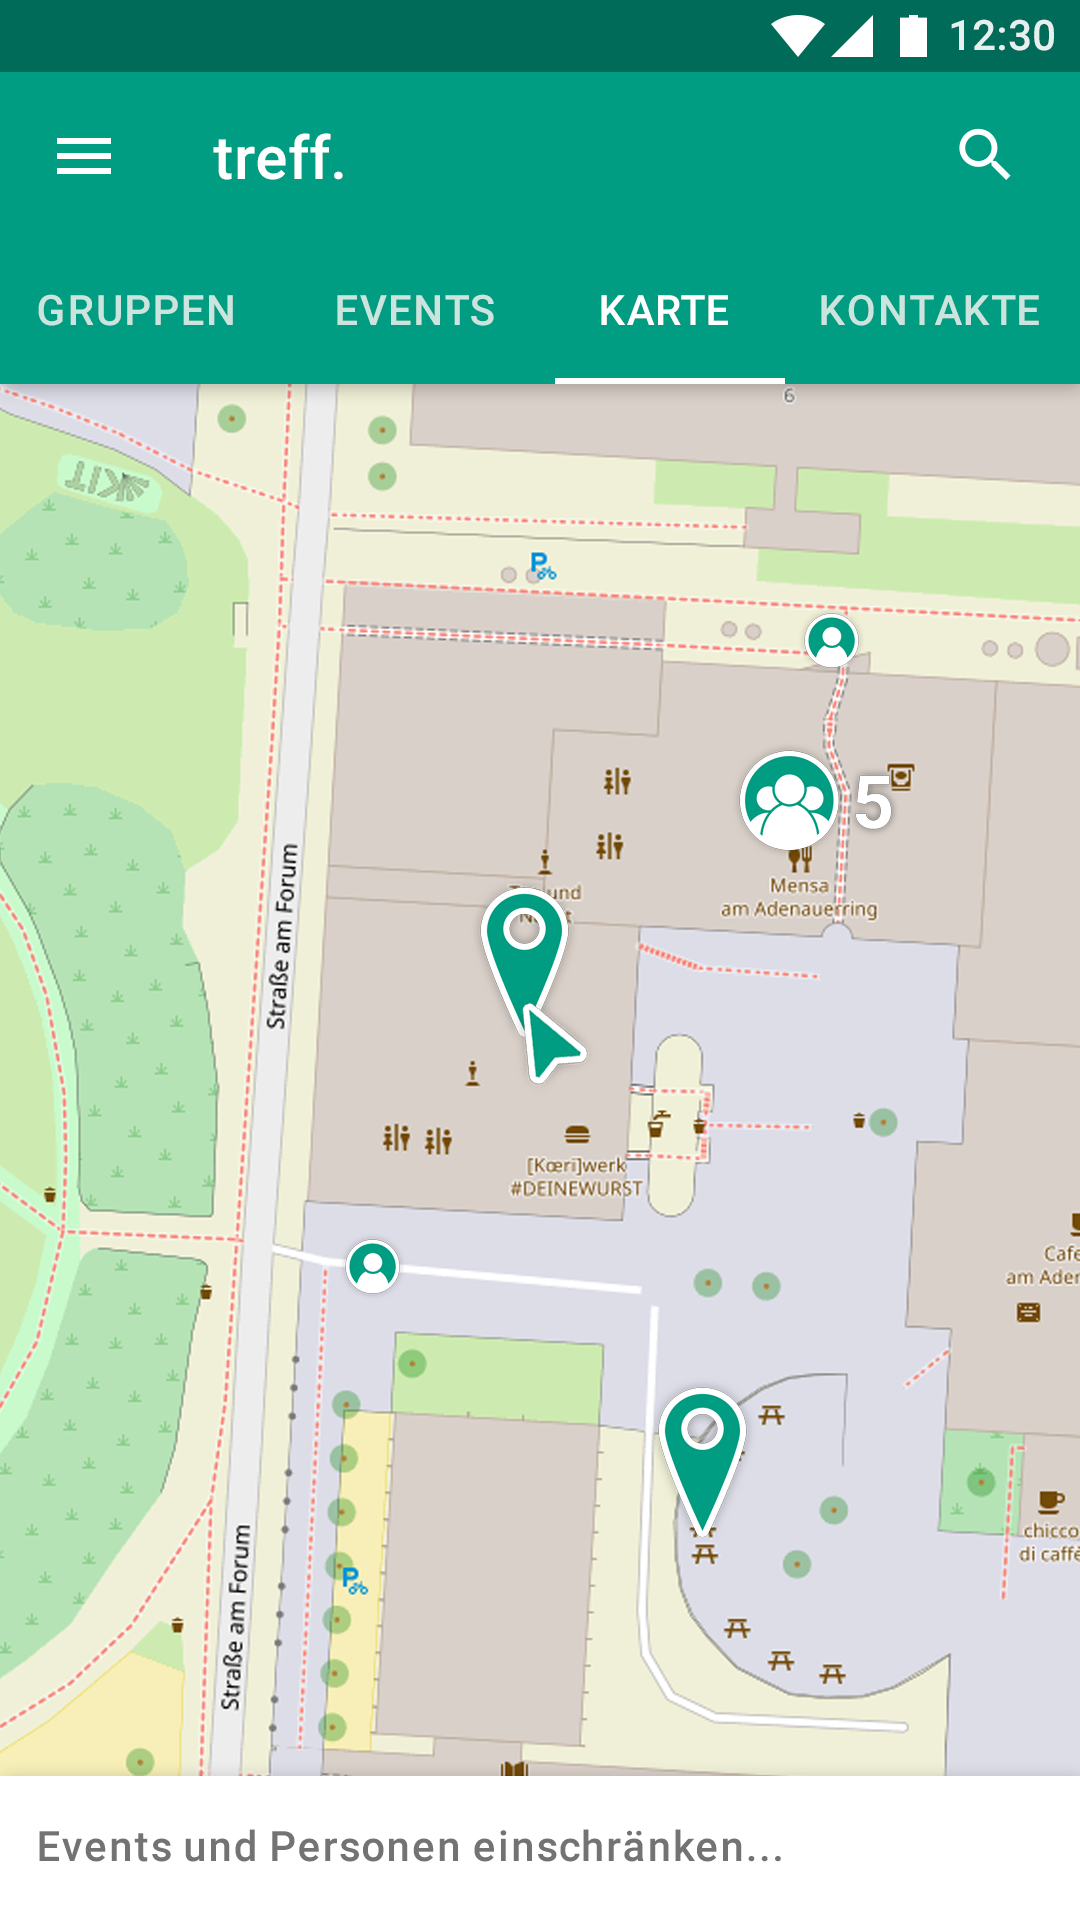
\includegraphics[width = 45mm]{images/gui-mockups/home_map.png}}
			\captionsetup{labelformat=empty}
			\centering
			\captionof{figure}{Umgebungskarte}
		\end{minipage}%
		\begin{minipage}{0.5\textwidth}
			\textbf{Streitpunkte}
			\begin{itemize}
				\setlength\itemsep{0.3em}
				\item[--] Gruppierungen mehrerer Standorte
				\item[--] Gruppenkarte vs Gesammtkarte
				\item[--] Filterfunktion
			\end{itemize}
		\end{minipage}%
	\end{frame}

	%%%%%%%%%%%%%%%%%%%%%%%%%%%%%%%%%%%%%%%%%%%%%%%%%%%%%

	\begin{frame}
		\begin{minipage}{0.5\textwidth}
			\setlength{\fboxsep}{0pt}% space between border and image
			\setlength{\fboxrule}{1pt}% width of border
			\fbox{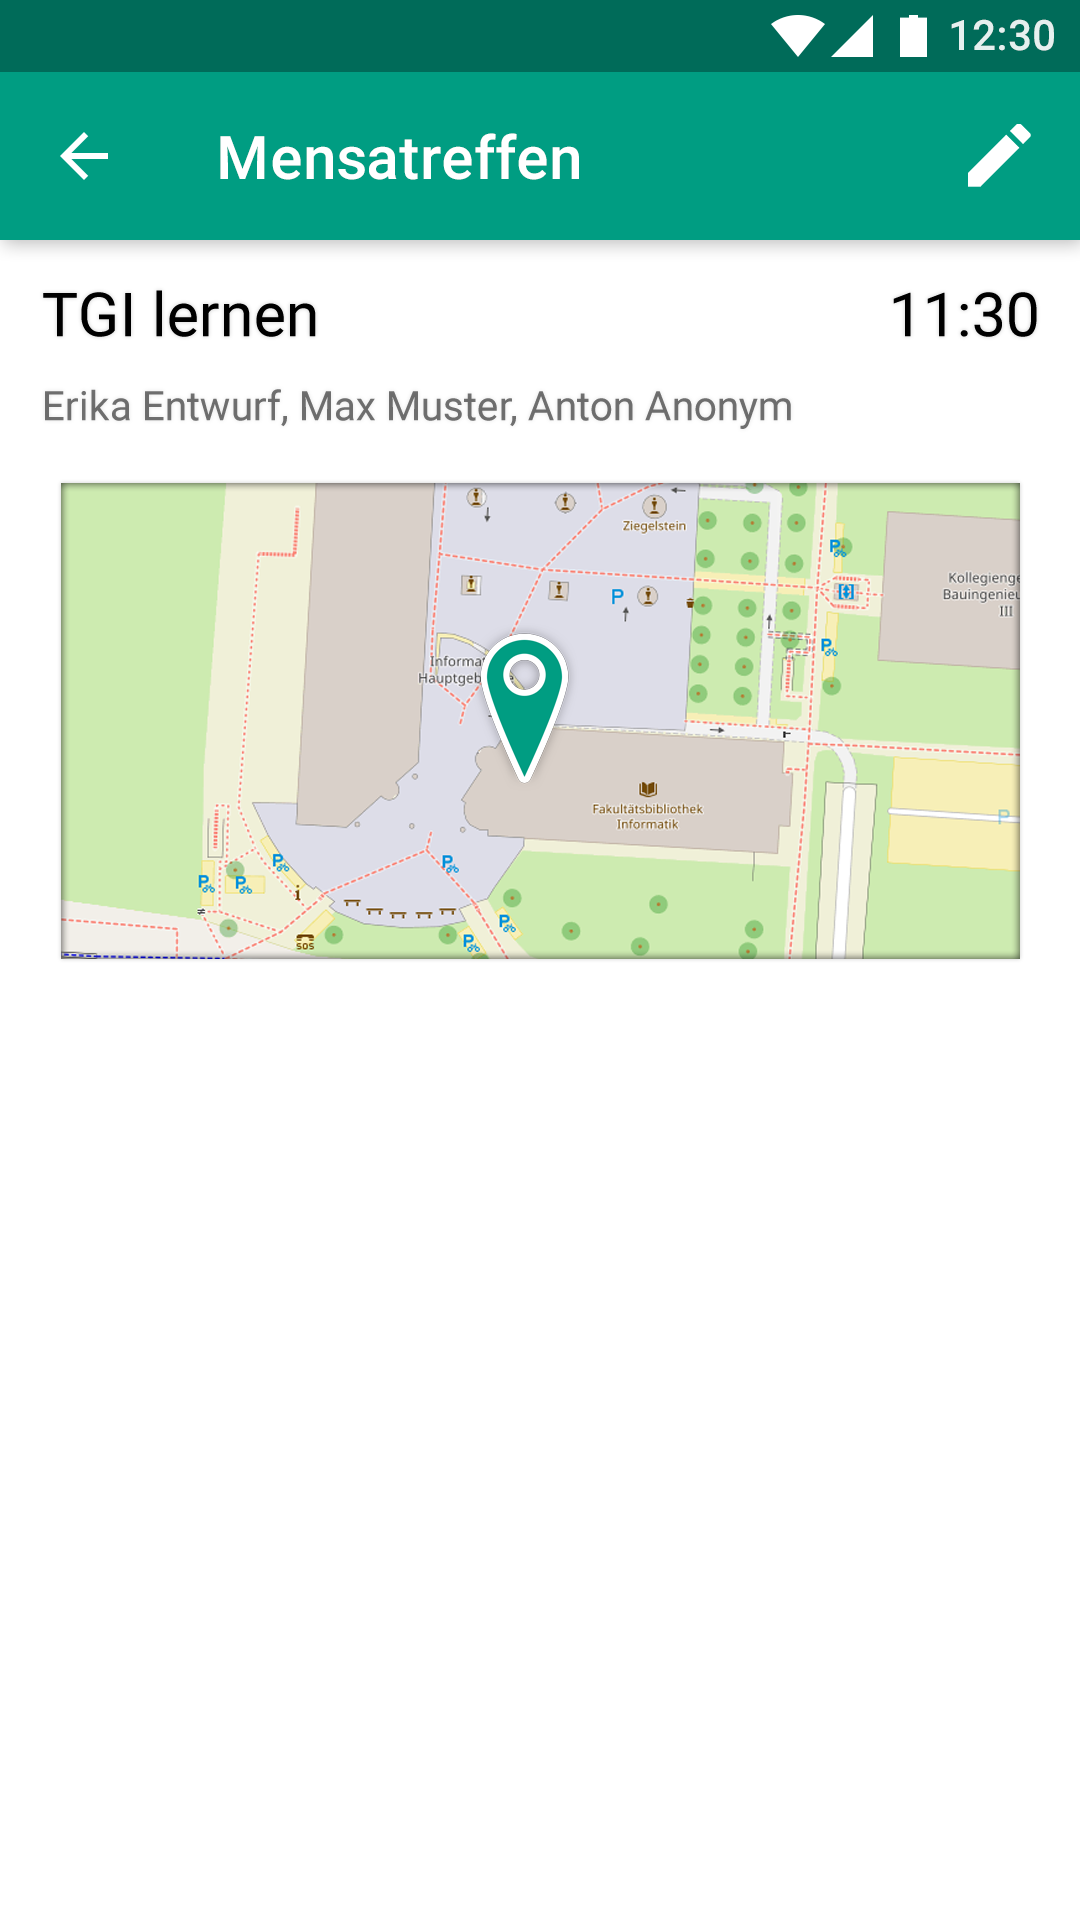
\includegraphics[width = 45mm]{images/gui-mockups/event.png}}
			\captionsetup{labelformat=empty}
			\centering
			\captionof{figure}{Liste aller Verabredungen einer Gruppe}
		\end{minipage}%
		\begin{minipage}{0.5\textwidth}
			\textbf{Verabredungen}
			\begin{itemize}
				\item[--] Fester Zeitpunkt und Ort
				\item[--] Für alle Mitglieder sichtbar
				\item[--] Benachrichtigung vor Beginn
			\end{itemize}
		\end{minipage}
	\end{frame}

\begin{frame}[plain]
\begin{minipage}{0.5\textwidth}
	\setlength{\fboxsep}{0pt}% space between border and image
	\setlength{\fboxrule}{1pt}% width of border
	\fbox{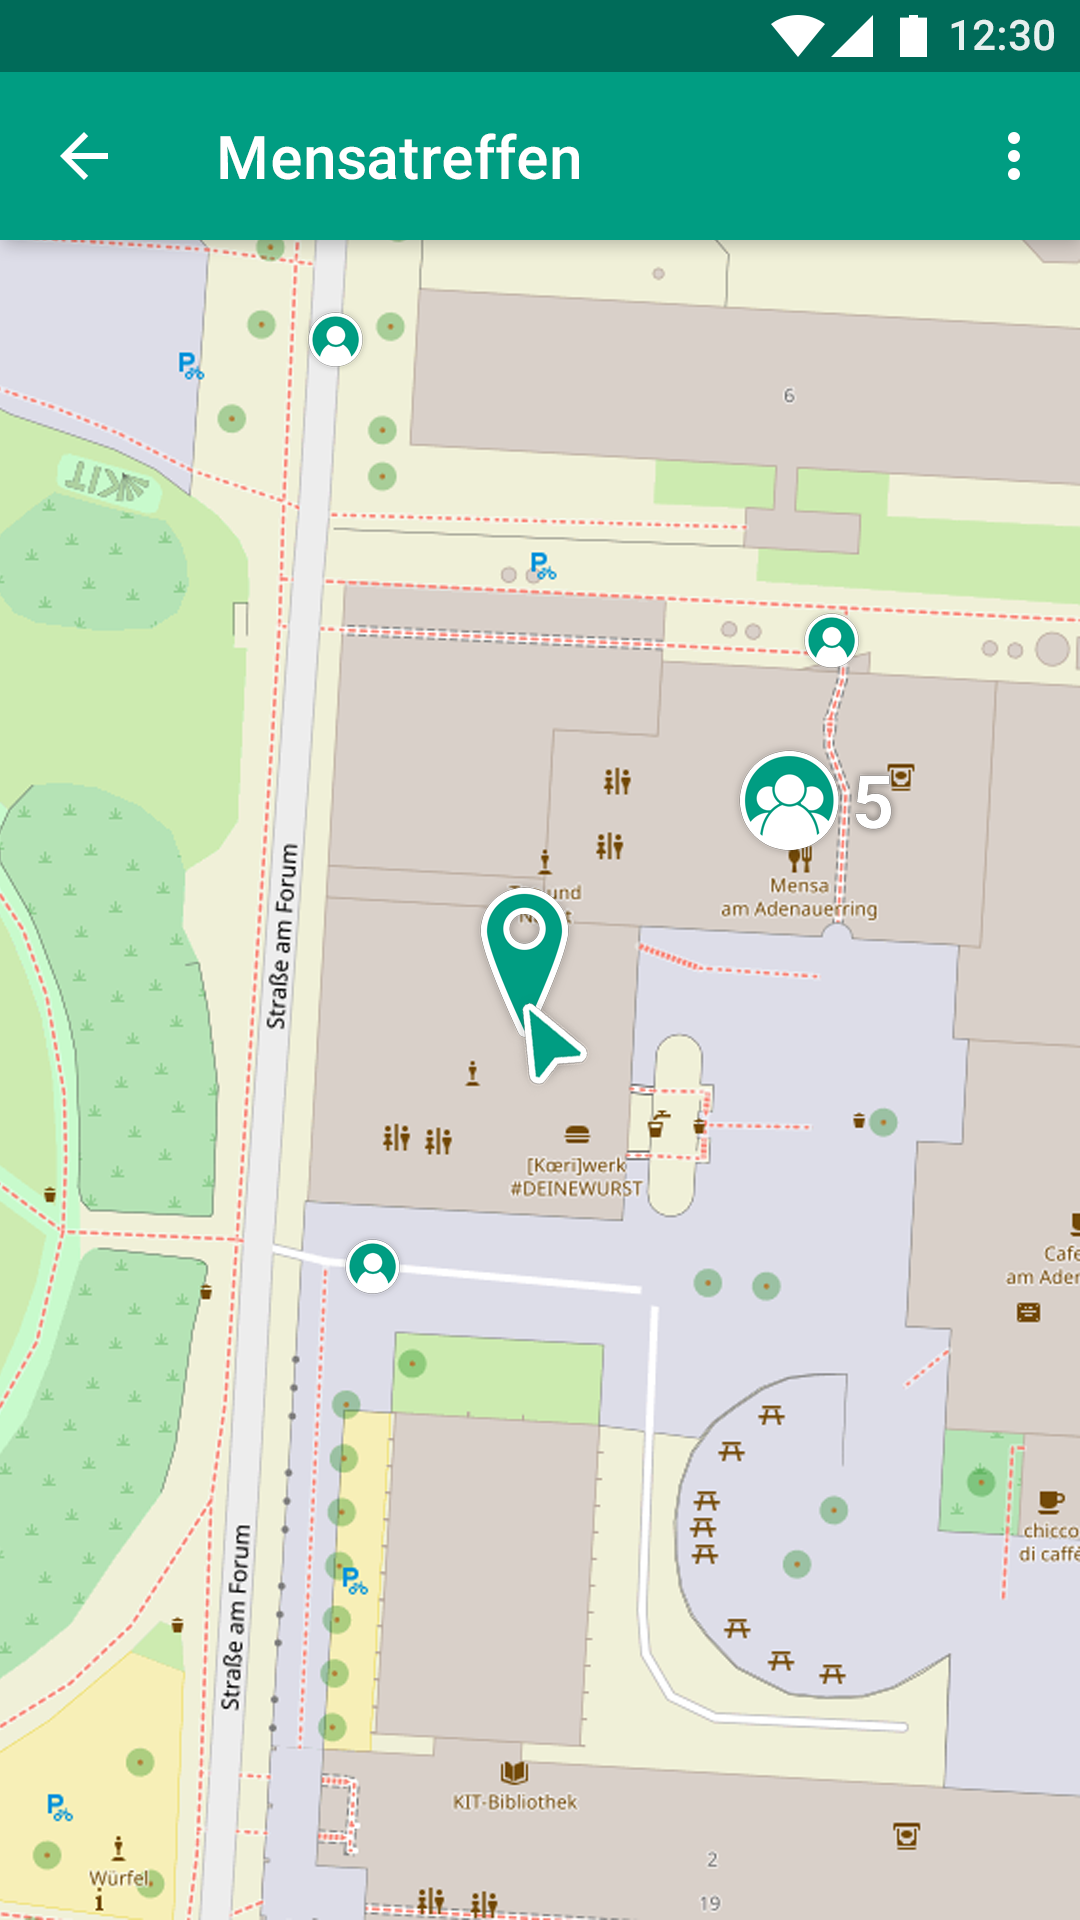
\includegraphics[width = 45mm]{images/gui-mockups/event_map.png}}
	\captionsetup{labelformat=empty}
	\centering
	\captionof{figure}{Umgebungskarte eines Gruppenmitglieds}
\end{minipage}%
\begin{minipage}{0.5\textwidth}
	\textbf{Verabredungen}
	\begin{itemize}
		\item[--] Fester Zeitpunkt und Ort
		\item[--] Für alle Mitglieder sichtbar
		\item[--] Benachrichtigung vor Beginn
	\end{itemize}
\end{minipage}
\end{frame}

\end{document}
